\newpage
\subsection{Disco}
Nesta secção apresentamos os procedimentos usados para desenvolver um disco. A motivação para o desenvolvimento desta figura provém da necessidade de representar os anéis planetários que rodeiam os planetas Saturno e Úrano.


\subsubsection{Análise do Problema}
O desenvolvimento do algoritmo para desenhar um disco foi feito usando como base o que já foi previamente feito para a esfera, não apresenta grandes dificuldade de compreensão dado a prática que já se teve com coordenadas polares até esta fase. 

Em análise ao que seria preciso fazer para se formar um disco, sempre se teve em mente que seria preciso representar duas circunferências, uma interior e outra exterior, querendo como produto final o preenchimento dos triângulos entre estas. O disco irá possuir um raio interior e um raio exterior. No entanto, chegou-se à conclusão que isto não era suficiente pois, desenhando o anel sem altura resulta que não seja visível de lado. A solução para isto foi desenhar mais duas circunferências com os mesmos pontos xx e zz mas com uma distancia fixa no eixo yy. 

\newpage
\subsubsection{Diagrama}

Nesta secção iremos começar por explicar graficamente o nosso disco, primeiramente, como já foi dito não se considerou existência de altura, e então o disco seria claramente explicado pelo seguinte diagrama. A seguir explica-se o processo com altura.

Decidimos manter este diagrama porque apesar de não considerar o fator altura é bastante esclarecedor em relação ao raciocínio e até ajuda o leitor a perceber passo a passo. 



\begin{center}
 	
 	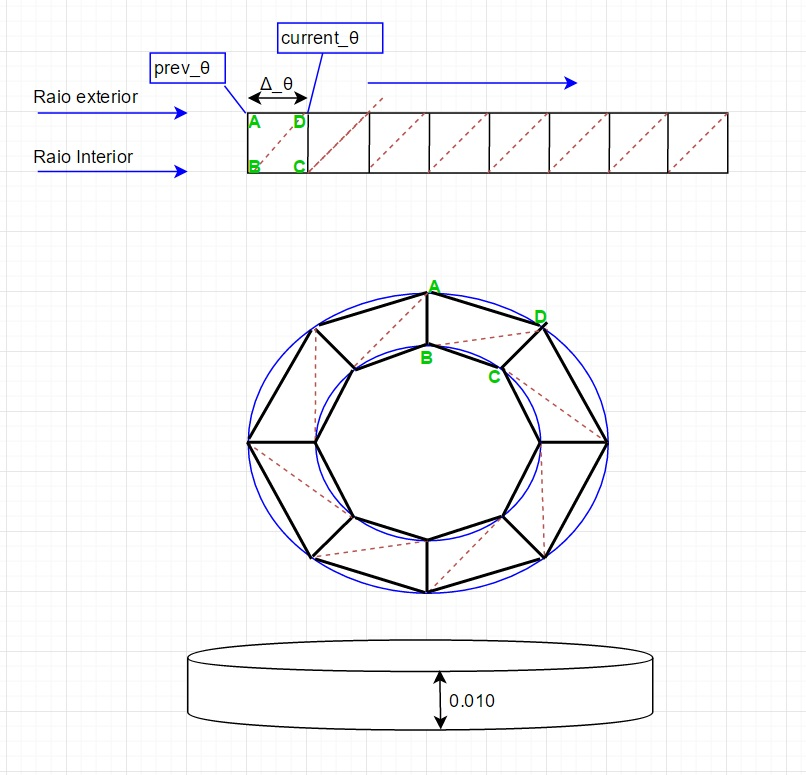
\includegraphics[width=\textwidth,height=\textheight,keepaspectratio]{resources/disco.jpg}
 	\captionsetup{type=figure, width=0.8\linewidth}
	\caption{Diagrama Disco}
\label{fig:ssec1:disc} 
\end{center}

Como se pode verificar o diagrama é relativamente semelhante ao da esfera. A matriz aqui observada apenas tem uma linha porque não se consideram \textit{stacks} na representação do disco. As 8 colunas que representam as 8 \textit{slices} (estas 8 slides servem meramente para propósitos exemplificativos). 

Como se pode observar, o raciocínio é desenhar quadricula a quadricula com dois triângulos cada, neste exemplo verifica-se que a primeira quadricula é constituída pelos triângulos ABD e BCD. As coordenadas de cada ponto (vértice dos triângulos) são calculados com o auxílio das variáveis angulares prev\_$\theta $ e current\_$\theta$ usando a formulação das coordenadas esféricas. A diferença entre esta é o comprimento/largura da quadricula que corresponde a \( \frac{2\Pi}{slices} \). 

Ora este processo é referente à face superior do disco. Para desenhar a face inferior faz-se o mesmo processo mas com outros vértices equivalentes nos eixos xx e zz mas com uma diferença fixa de 0.010 yy para representar a altura.

Quanto à face lateral do disco o processo é idêntico ao representado na matriz acima, mas enquanto que, para representar tanto a face superior como a inferior, os pontos usados têm todos os o mesmo valor yy, para representar o lado do disco usa-se uma combinação dos pontos de ambas as faces. 





\subsubsection{Figura}

\subsubsection{Algoritmo}

\begin{algorithm}
\floatname{algorithm}{Algoritmo}
\caption{Disco}\label{alg:sec1:disco}
\begin{algorithmic}[1]
\State $\Delta\_\theta \gets \dfrac{2\pi}{slices}$


\State $prev\_\theta \gets 0$
\State $current\_\theta \gets \Delta\_\theta$

\State $i \gets 0$
\While{$i \leq slices$} 

\State $Ponto A \gets raioOut*\sin(prev\_\theta),
\newline 0.005,
\newline raioOut*\cos(prev\_\theta)$

\State $Ponto B \gets raioIn*\sin(prev\_\theta),
\newline 0.005,
\newline raioIn*\cos(prev\_\theta)$

\State $Ponto C \gets raioIn*\sin(current\_\theta),
\newline 0.005,
\newline raioIn*\cos(current\_\theta)$

\State $Ponto D \gets raioOut*\sin(current\_\theta),
\newline  0.005,
\newline raioOut*\cos(current\_\theta)$

\State $Ponto A2 \gets raioOut*\sin(prev\_\theta),
\newline -0.005,
\newline raioOut*\cos(prev\_\theta)$

\State $Ponto B \gets raioIn*\sin(prev\_\theta),
\newline -0.005,
\newline raioIn*\cos(prev\_\theta)$

\State $Ponto C \gets raioIn*\sin(current\_\theta),
\newline -0.005,
\newline raioIn*\cos(current\_\theta)$

\State $Ponto D \gets raioOut*\sin(current\_\theta),
\newline  -0.005,
\newline raioOut*\cos(current\_\theta)$

\State $i \gets i + 1$ 

\State $Triangulo(Ponto A2, Ponto B2, Ponto D2)$
\State $Triangulo(Ponto D2, Ponto B2, Ponto C2)$

\State $Triangulo(Ponto D, Ponto B, Ponto A)$
\State $Triangulo(Ponto C, Ponto B, Ponto D)$

\State $Triangulo(Ponto A2, Ponto A, Ponto D2)$
\State $Triangulo(Ponto D2, Ponto A2, Ponto A)$

\State $prev\_\theta \gets Current\_\theta$
\State $current\_\theta \gets Current\_\theta + \Delta\_\theta$



\EndWhile
\end{algorithmic}
\end{algorithm}